\documentclass[11pt,a4paper]{article}
\usepackage[margin=1in]{geometry}
\usepackage{booktabs}
\usepackage{graphicx}
\usepackage{hyperref}
\usepackage{float}
\usepackage{caption}
\usepackage{setspace}
\setstretch{1.1}

\title{AI651 Assignment 1 Report}
\author{Muhammad Tayyab Tahir Qureshi\\Roll number 25280024\\Lahore University of Management Sciences}
\date{Fall 2026}

\begin{document}
\maketitle

\noindent\textbf{Name:} Muhammad Tayyab Tahir Qureshi\\
\noindent\textbf{Roll number:} 25280024\\
\noindent\textbf{GitHub repository (public):}
\url{https://github.com/ttqureshi/DL4STG-PA1}

\vspace{0.5em}
\noindent This report covers Task 1 and Task 2. Task 2 code is \texttt{Task2/Task2.ipynb}.

\section*{Task 1}

\noindent\textbf{Run setting used for the Task 1 numbers:}
\texttt{PA1\_PRESET=full}, seed 0, CUDA (Tesla T4). Context length $L=96$, horizon $H=48$.
Validation numbers are on the established stations (1--3) or held-out station 4, as named in each table.
Figures come from the notebook Outputs folder in the repository.

\section*{What I implemented}
\begin{enumerate}
  \item \texttt{RawAttentionForecaster.forward}: embed context, add position, run Attention blocks, flatten, forecast head.
  \item \texttt{SeriesDecomposition.forward}: centered moving average with replicate padding; return (remainder, trend).
  \item \texttt{aggregate\_delays}: weighted circular shifts, $z[t]=\sum_j w_j\,v[(t-d_j)\bmod L]$.
\end{enumerate}

\section{Response 1A}
\subsection*{Expected order before Output 1.1}
I expected:
\begin{enumerate}
  \item Established: Period-routed ridge $>$ Sensor-specific ridge $>$ Shared ridge $>$ Raw Attention.
  \item Held-out station 4: Period-routed ridge $>$ Shared ridge $>$ Raw Attention (Sensor-specific has no fit for station 4).
\end{enumerate}
Reason: the line changes pace by product, so a map that knows the period should beat one shared matrix. I thought Raw Attention would need more data or tuning before it beats a closed-form linear baseline.

\subsection*{Measured order (Output 1.1, validation)}
\begin{table}[H]
\centering
\small
\begin{tabular}{lrrrr}
\toprule
Model & Est.\ RMSE & Est.\ MSE & Held-out RMSE & Params \\
\midrule
Period-routed ridge & 0.166 & 0.028 & 0.173 & 59904 \\
Raw Attention & 0.430 & 0.184 & 0.629 & 368368 \\
Shared ridge & 0.767 & 0.588 & 0.876 & 4608 \\
Sensor-specific ridge & 0.768 & 0.590 & --- & 13824 \\
\bottomrule
\end{tabular}
\caption{Output 1.1 summary. RMSE in m/s$^2$, MSE in (m/s$^2$)$^2$.}
\end{table}

Revised order:
\begin{enumerate}
  \item Established: Period-routed ridge $\gg$ Raw Attention $>$ Shared ridge $\approx$ Sensor-specific ridge.
  \item Held-out: Period-routed ridge $\gg$ Raw Attention $>$ Shared ridge.
\end{enumerate}

What changed: Raw Attention clearly beats both non-routed ridge models (about 0.43 vs 0.77 RMSE on established stations). My early guess that Attention would stay last was wrong. Period-routed ridge is still far ahead (0.17 RMSE). Across products A/B/C the same ranking holds; Product B is a bit harder for Raw Attention (0.45 RMSE) than A/C.

Why this matches the model assumptions:
\begin{itemize}
  \item Shared ridge fits one linear map for every pace, so it has to compromise when Product A ($\sim$16-sample cycle) and Product C ($\sim$30-sample cycle) need different phases.
  \item Sensor-specific ridge helps only a little here; the hard part is pace, not station identity alone.
  \item Period-routed ridge picks a map by estimated period, which matches the generator (one actual pace per operating run).
  \item Raw Attention builds mixing weights from the context, so it can adapt without an explicit period feature, but it is still worse than giving the linear model the period directly.
\end{itemize}

\section{Response 1B}
Output 1.2 compares Station 1 under Product A (period $\approx 16.1$) and Product C (period $\approx 30.1$). Shared ridge RMSE jumps around between those two windows (about 0.78 on A vs 0.45 on C in the shown cases). One fixed $\hat W$ cannot keep the right phase for both spacings. On the faster Product A window the shared forecast looks phase-shifted relative to the true vibration; on the slower Product C window the shape mismatch is smaller but still there. Period-routed ridge stays much closer in both windows (about 0.23 and 0.15 RMSE).

\begin{figure}[H]
\centering
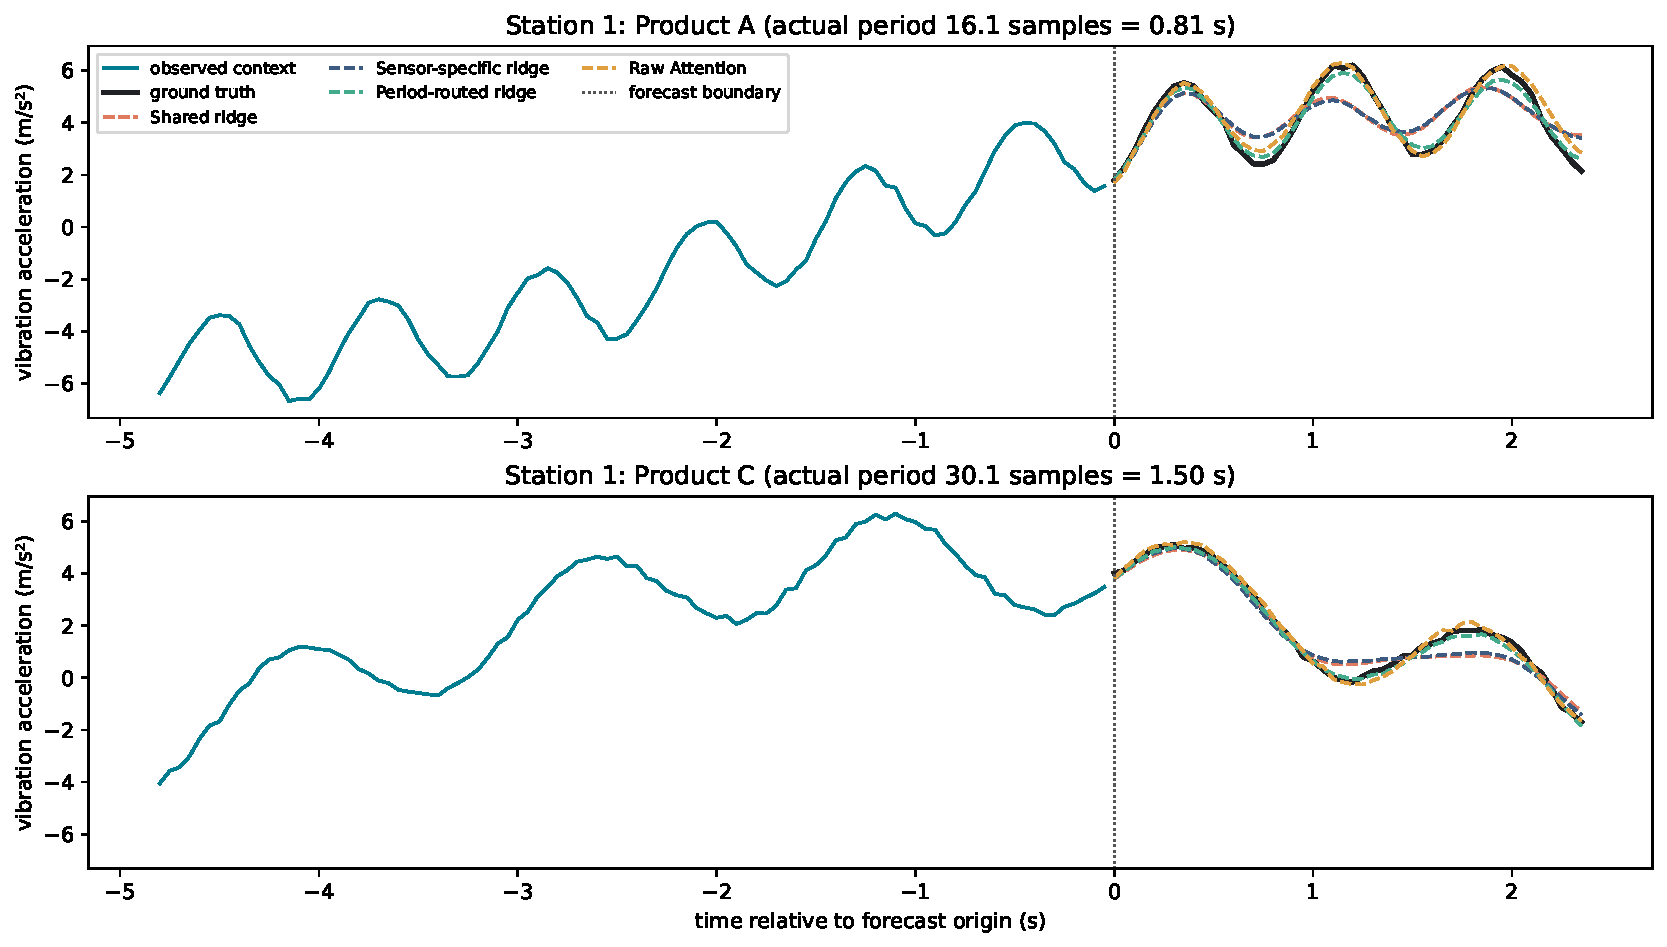
\includegraphics[width=0.95\textwidth]{Task1/results/design/1.2-1.pdf}
\caption{Output 1.2: same station, two products.}
\end{figure}

Output 1.3 compares Attention weights for those two contexts. Mean absolute weight difference is about 0.012 and the max difference is about 0.43. So the same learned $W_Q,W_K,W_V$ produce different mixing for different inputs. Ridge cannot do that: $\hat W$ is fixed after fitting. I am not reading Output 1.3 as ``Attention found the physical period.'' It only shows that mixing depends on context.

\begin{figure}[H]
\centering
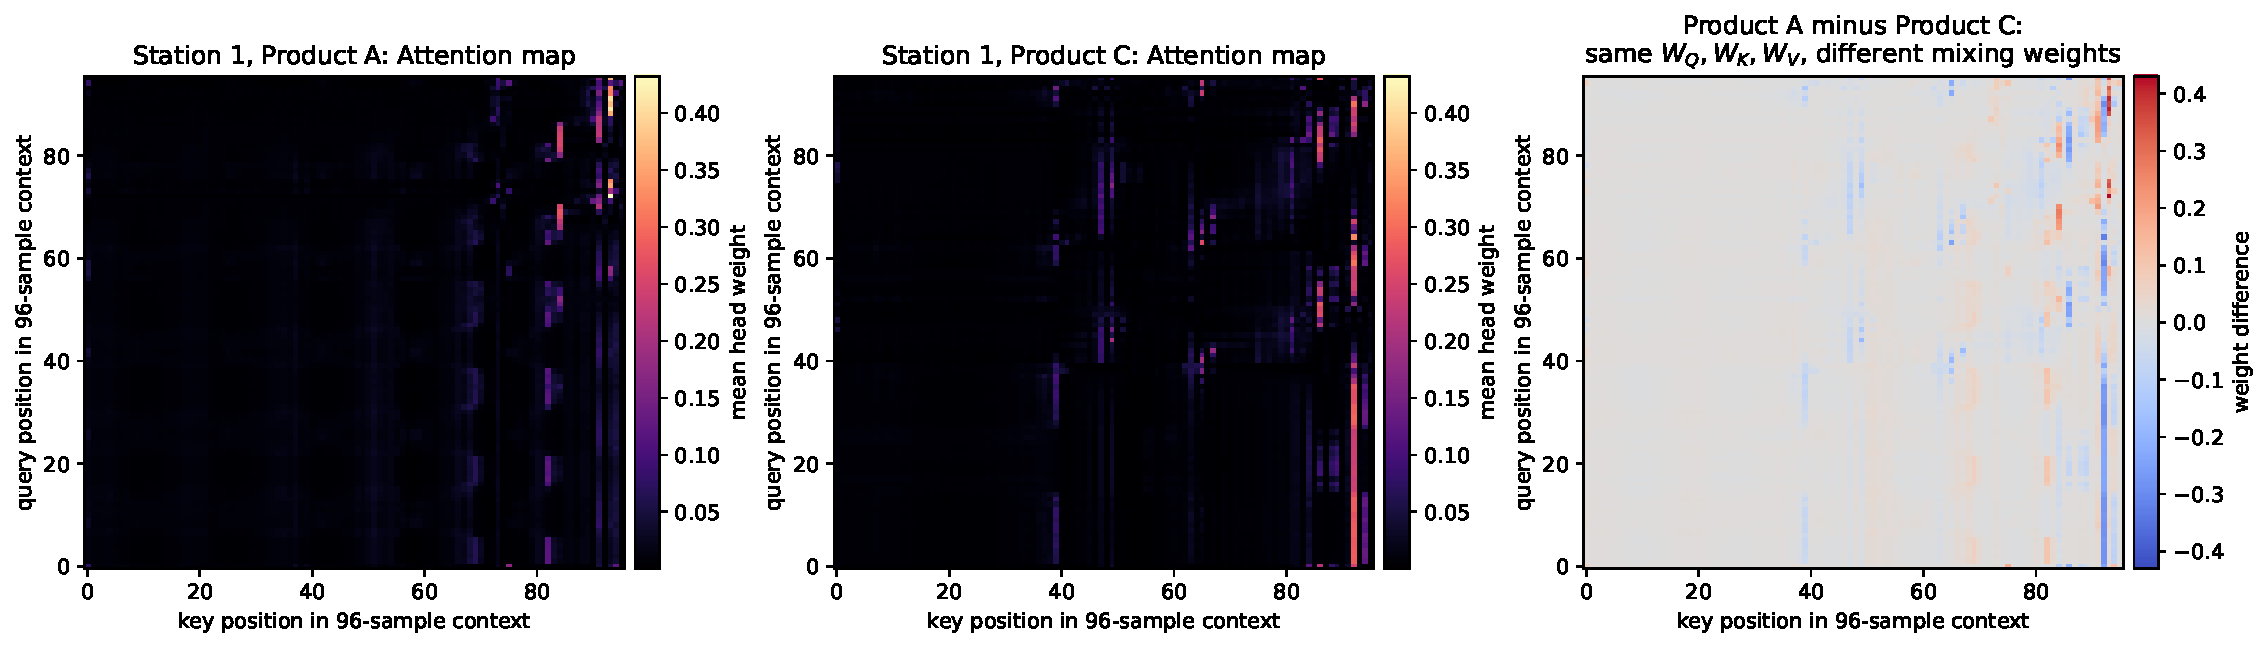
\includegraphics[width=0.95\textwidth]{Task1/results/design/1.3-1.pdf}
\caption{Output 1.3: Attention weight difference across two contexts.}
\end{figure}

\section{Response 2}
I implemented centered moving-average decomposition with replicate padding at the ends.

Selected width: \textbf{41} (from Outputs 2.1--2.2). Wider widths push more energy into the residual and improve oracle period recovery. Width 41 has the highest recovery within one sample (0.998) among the candidates. Visually in Output 2.1, width 41 leaves a residual with clearer oscillation and a smoother trend than width 17.

\begin{figure}[H]
\centering
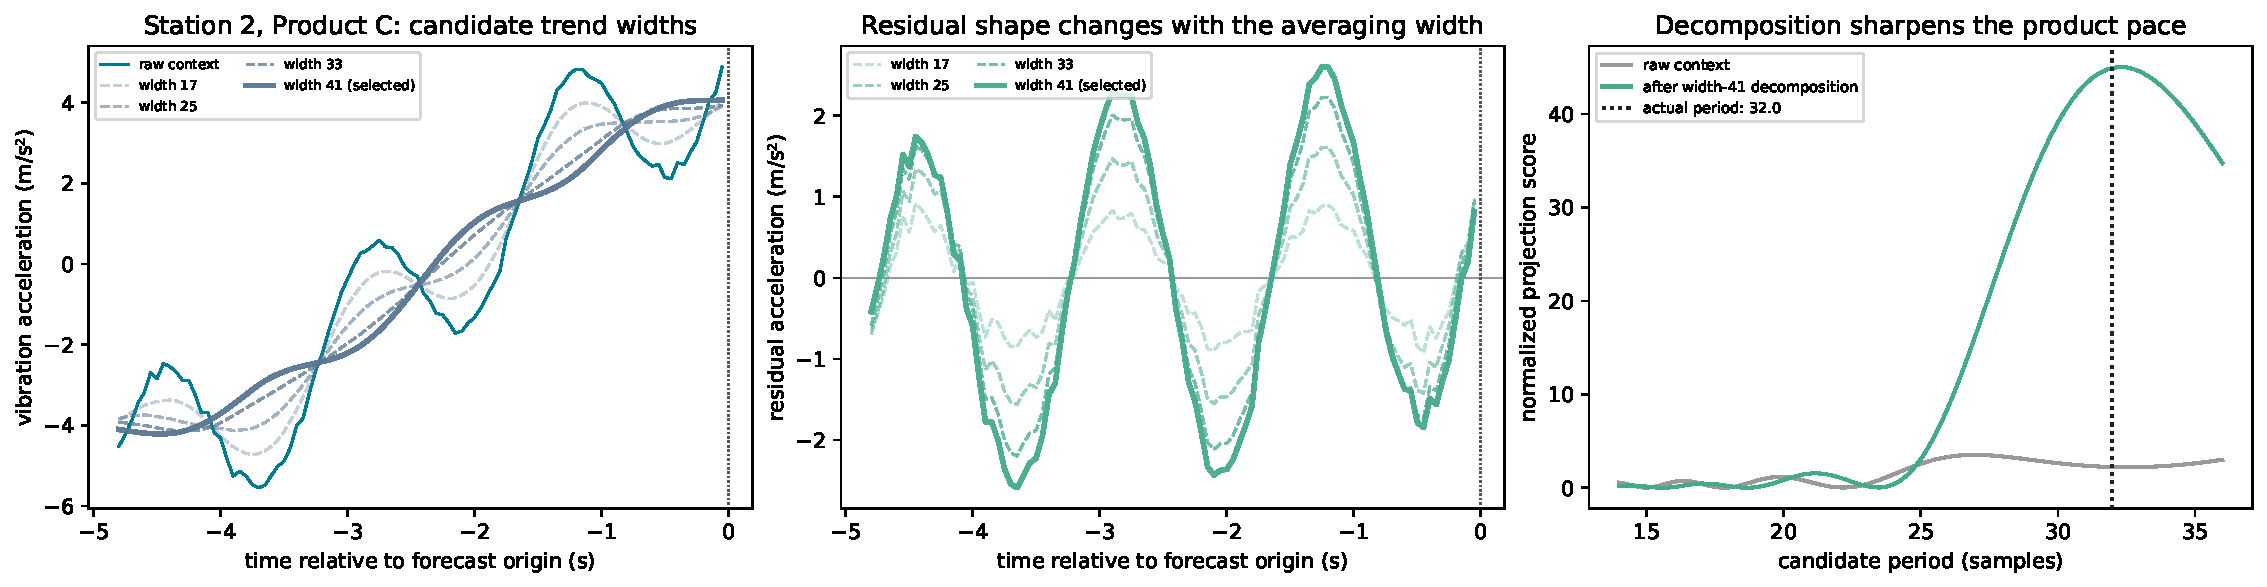
\includegraphics[width=0.85\textwidth]{Task1/results/design/2.1-1.pdf}
\caption{Output 2.1: trend/residual for candidate widths.}
\end{figure}

\begin{figure}[H]
\centering
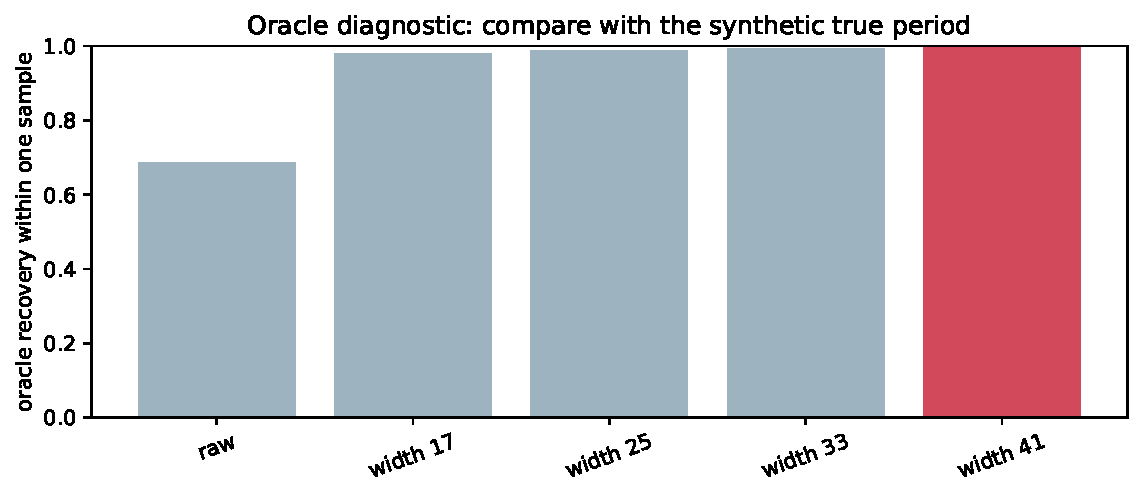
\includegraphics[width=0.7\textwidth]{Task1/results/design/2.2-1.pdf}
\caption{Output 2.2: oracle period recovery vs width.}
\end{figure}

Output 2.3 (validation RMSE):
\begin{itemize}
  \item Established, Raw Attention $\approx 0.42$--$0.45$ by product.
  \item Established, Attention + decomposition $\approx 0.28$--$0.36$ by product.
\end{itemize}
So splitting helps. Held-out also improves (for example Product A: 0.64 $\to$ 0.40).

Why a moving average fits this world: drift is slow ($\sim$240 samples) and vibration is faster (14--36). A mid-range odd window can soak up the ramp while leaving most of the cycle in the remainder. The training-only oracle in Output 2.2 is useful because we can check whether the residual still reveals the known period before we trust the width for forecasting. It is not an input to the deployed model.

Where this bias fails: if the ``trend'' has a sharp step inside the context, a centered average smears the step into nearby samples and pollutes the residual. An alternative would be a causal low-pass filter (only past samples). That avoids peeking at future samples inside the window, but the edge behavior and phase lag would change.

\begin{figure}[H]
\centering
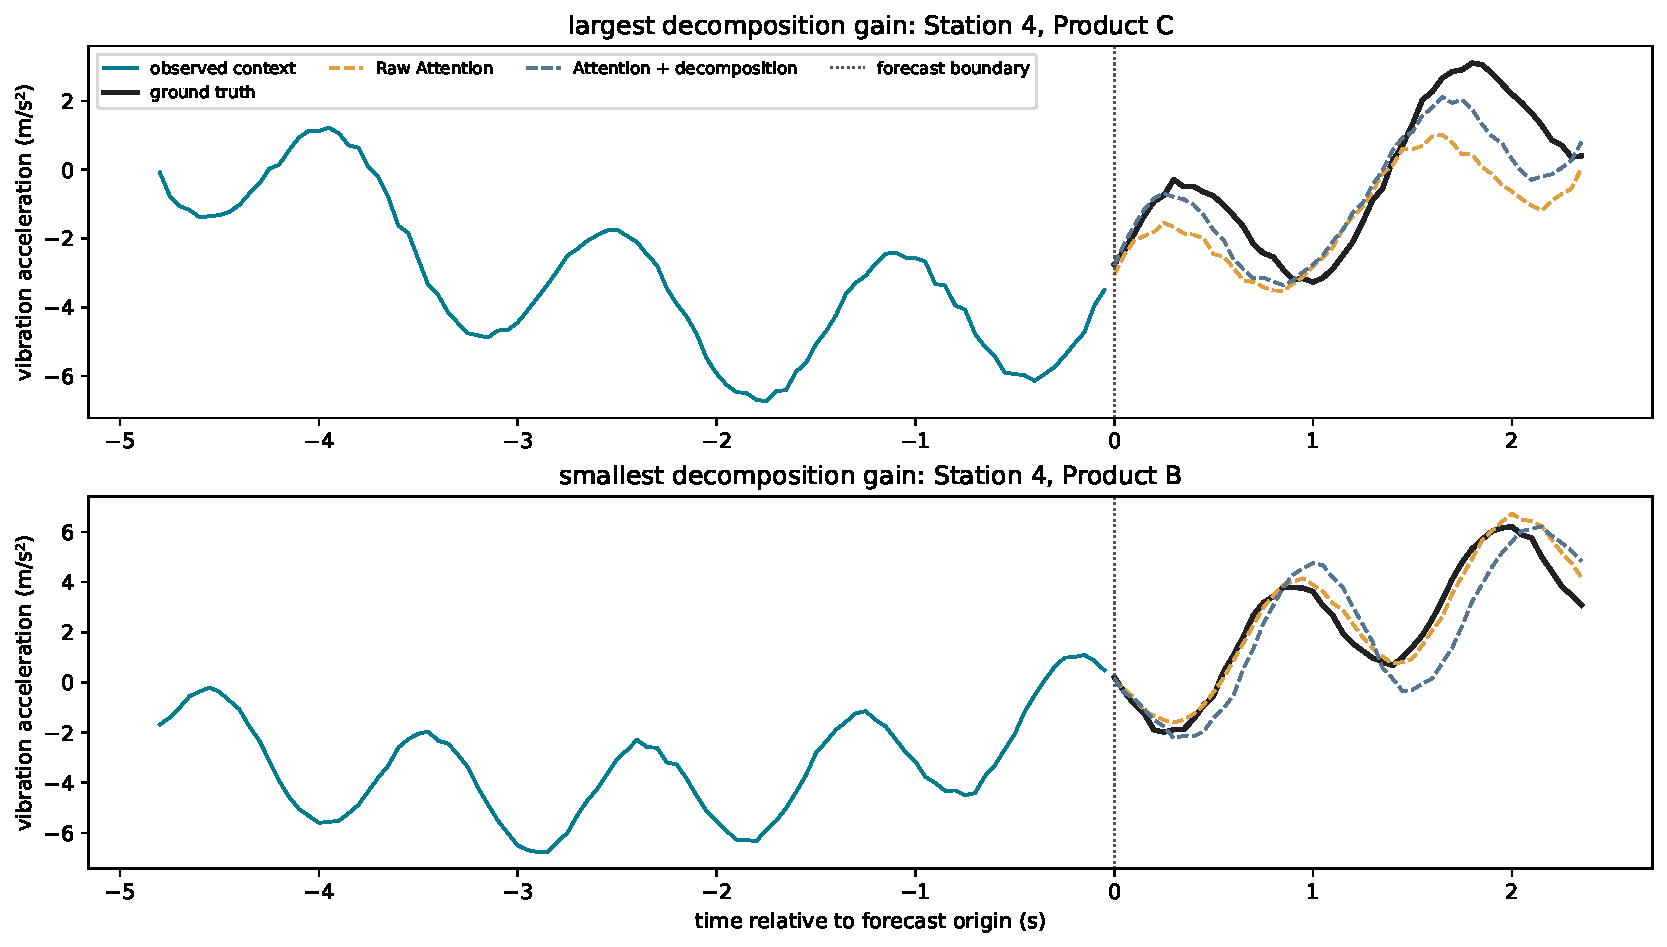
\includegraphics[width=0.85\textwidth]{Task1/results/design/2.3-1.pdf}
\caption{Output 2.3: decomposition ablation forecasts.}
\end{figure}

\section{Response 3}
I implemented \texttt{aggregate\_delays}. The worked example with $v=[10,20,30,40]$, delays $[1,3]$, weights $[0.75,0.25]$ gives $z_0=35$, so the shift direction $(t-d)\bmod L$ is correct. Output 3.1 also matches FFT delay scores to the direct circular correlation on $[1,3,1,3]$.

Output 3.2 (signal-level diagnostic, not learned mixer scores): for Station 2, Product A, the strongest residual correlations sit at delay 16 and 32. The run period is $P\approx 16.13$, so those peaks are $P$ and $2P$.

\begin{figure}[H]
\centering
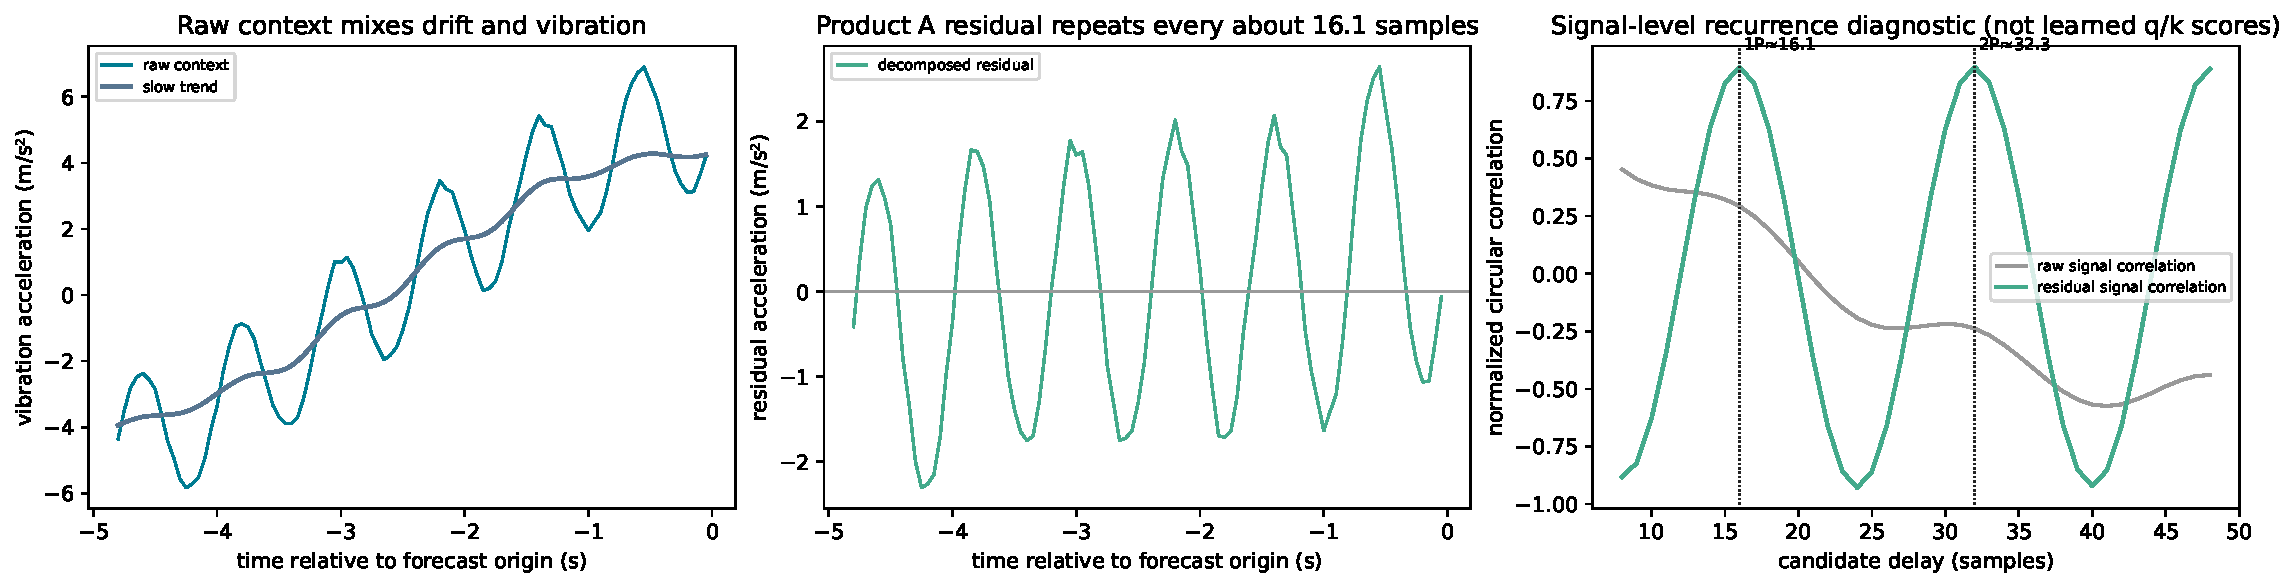
\includegraphics[width=0.75\textwidth]{Task1/results/design/3.2-1.pdf}
\caption{Output 3.2: recurrence after removing slow structure.}
\end{figure}

Why decomposition helps delay evidence: a rising ramp looks similar to itself after many shifts, so raw circular correlation is muddy. After removing the slow part, peaks near $P$ and $2P$ stand out. That supports organizing mixing by a few recurring delays instead of every position pair.

When delay mixing is the wrong bias: a one-off transient (jam spike) that does not repeat inside the context. High scores would latch onto some lag that is not a real cycle, and the forecast would copy the wrong past segment.

\section{Response 4}
\subsection*{(a) Prediction before Output 4.1}
When the slow ramp is large, decomposition should help more than changing the mixer, because it sends the ramp to a linear trend head and keeps Attention/delay focused on the residual vibration.

\subsection*{(b) Four neural models and baselines (validation, established)}
\begin{table}[H]
\centering
\small
\begin{tabular}{lrrr}
\toprule
Model & RMSE & MSE & Fit s \\
\midrule
Period-routed ridge & 0.166 & 0.028 & 0.02 \\
Autoformer-inspired & 0.198 & 0.039 & 107 \\
Raw delay mixer & 0.220 & 0.048 & 90 \\
Attention + decomposition & 0.314 & 0.098 & 89 \\
Raw Attention & 0.430 & 0.184 & 75 \\
Shared ridge & 0.767 & 0.588 & 0.03 \\
\bottomrule
\end{tabular}
\caption{Output 4.1 / 1.1 validation on established stations.}
\end{table}

Switch effects from Raw Attention (0.430 RMSE): delay alone $\to$ 0.220; decomposition alone $\to$ 0.314; both $\to$ 0.198. The combined gain (0.232) is less than the sum of the separate gains (0.210+0.116=0.326), so the two upgrades overlap. Delay helps more than decomposition alone in this run. Output 4.2 shows RMSE rising with horizon for all models; period-routed ridge stays lowest across the 48 steps, and Autoformer-inspired is the best neural curve.

\begin{figure}[H]
\centering
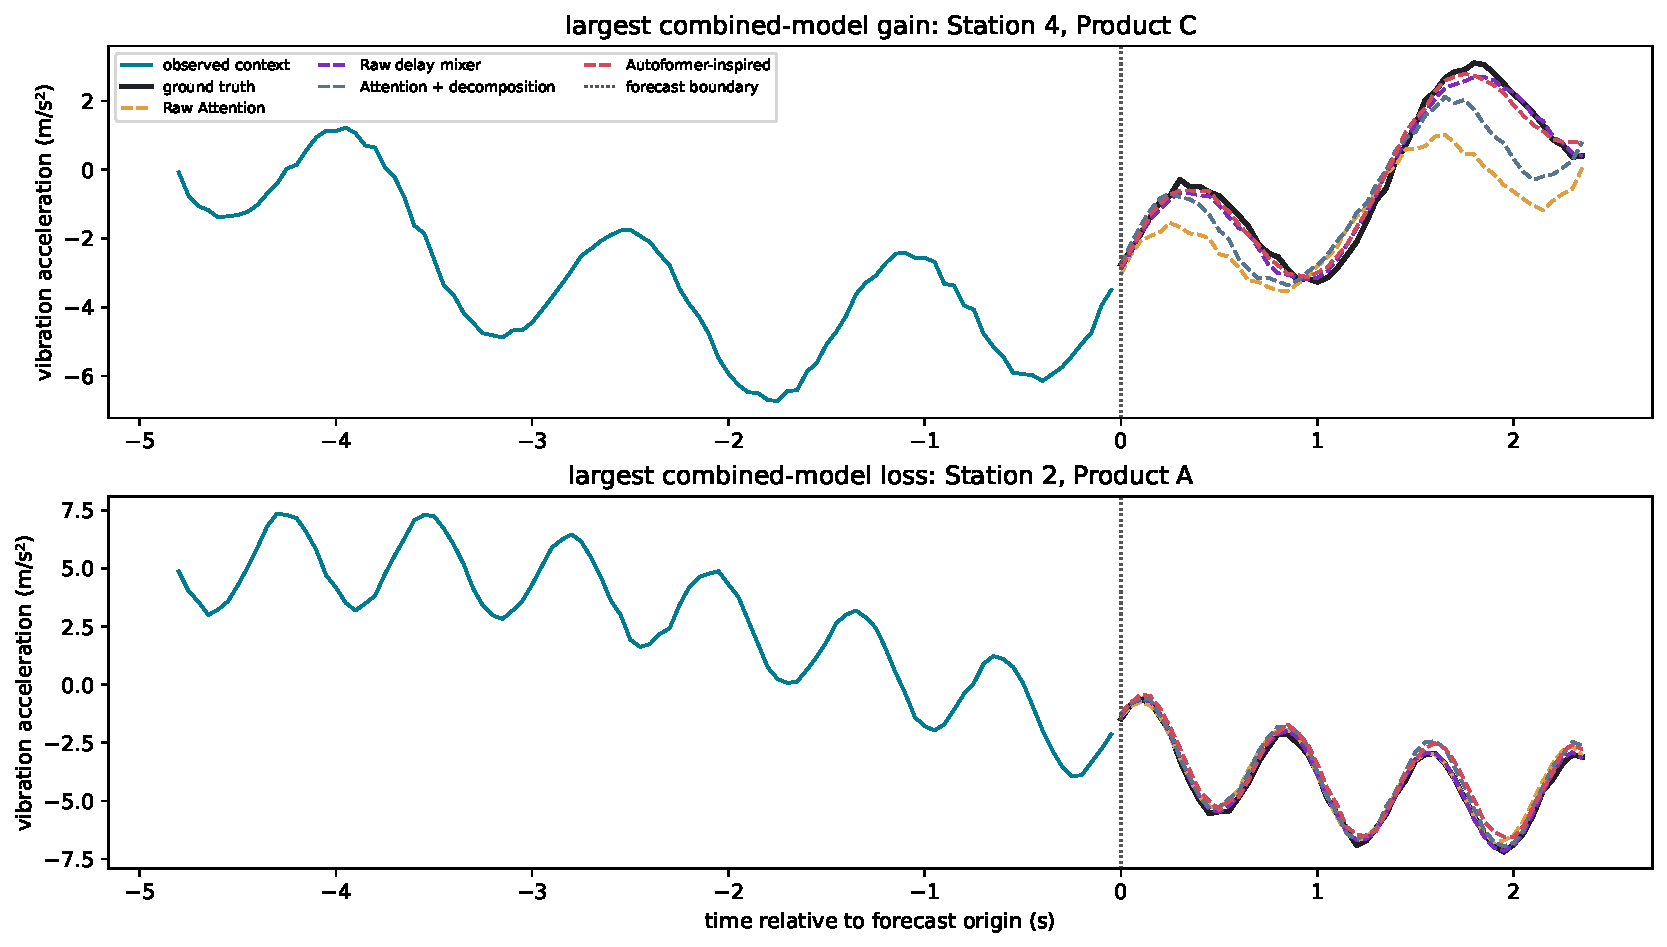
\includegraphics[width=0.95\textwidth]{Task1/results/design/4.1-1.pdf}
\caption{Output 4.1: model comparison and example forecasts.}
\end{figure}

\begin{figure}[H]
\centering
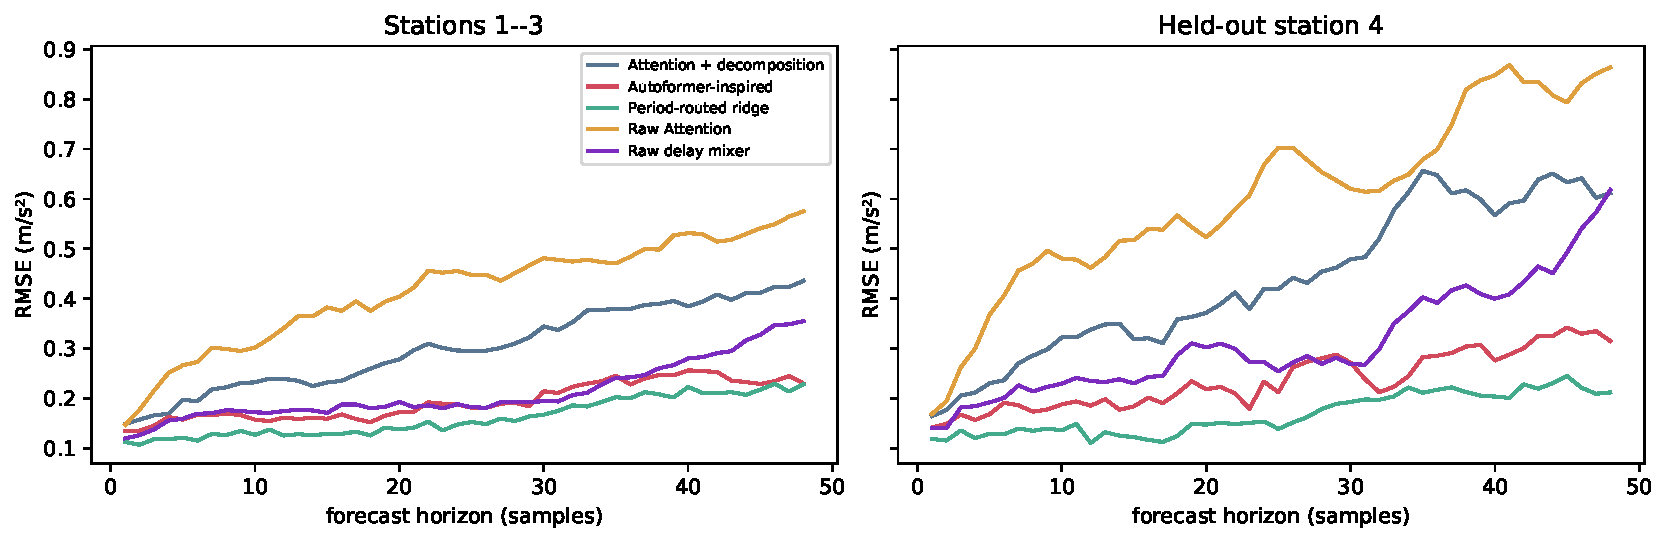
\includegraphics[width=0.95\textwidth]{Task1/results/design/4.2-1.pdf}
\caption{Output 4.2: error vs forecast horizon.}
\end{figure}

\subsection*{(c) Deployment choices}
I deploy \textbf{Period-routed ridge} for established stations and for held-out station 4.
\begin{itemize}
  \item Best validation RMSE on both groups (0.166 and 0.173).
  \item Tiny cost: about 60k parameters and under 0.1 s fit, vs $\sim$370k parameters and $\sim$75--107 s for the neural models.
  \item Sensor-specific ridge is invalid for station 4.
\end{itemize}
Test check (Output 4.3): established test RMSE 0.161, held-out test RMSE 0.183. Close to validation, so the choice did not overfit the validation split.

\textbf{Response 4 interpretation (short).}
Both switches help, delay more than decomposition, and stacking them helps less than adding the two gains. Still, a linear model that is told the period beats every neural option here. Extra flexibility did not beat the right inductive bias on this benchmark.

\section*{Task 2. Next 168 steps}

The code is \texttt{Task2/Task2.ipynb}. It forecasts \texttt{time\_idx} 43657 through 43824. The submitted model is an Autoformer. It uses a moving-average decomposition and an auto-correlation block, adapted from Wu et al., NeurIPS 2021 (\url{https://github.com/thuml/Autoformer}). I did not copy that repository. Both mechanisms run in the forward pass.

\subsection*{Data and how I scored it}

The training file has 43,656 points on a regular grid and no missing values. The optional file has columns A to J at every time step, including the horizon. The assignment allows those future covariates, so using them is not leakage.

A, B, and C are standardized. D, E, and F are skewed, so I take $\log(1+x)$ and then standardize. G to J already sum to one on every row, so I leave them as they are. The target is standardized on the fit portion. Forecasts are mapped back and clipped at zero, because the series never goes negative.

Validation is the last 12 blocks of 168 steps. They do not overlap. During the comparison, nothing after the start of that region is used to fit the scalers or the weights. Each setting is repeated with seeds 0, 1, and 2.

On those blocks, predicting the training mean gets RMSE 109.10. Repeating the last value gets 173.98. Repeating the last day gets 153.21. A model has to beat the mean before it is worth keeping.

\subsection*{The model}

Decomposition is a moving average of length 25. The seasonal part is the residual.

Auto-correlation follows the paper. Queries, keys, and values are linear maps of the window. An FFT picks the lags that line up, and the top $k$ of them are mixed, with $k$ about $3\ln L$. On a window of 168 that is 15 delays, so the daily lag is kept. Training and prediction use the same top-$k$ path.

The Autoformer itself is small: width 32, one encoder layer, one decoder layer. Its seasonal output starts at zero and is added as a residual.

Each of the 168 steps also has its own feature vector, built only from history before the forecast origin. It holds the last value, the mean of the last 24 steps, the mean of the last 168 steps, the same clock hour from the last observed day, the value one week before the target step, sine and cosine of the hour and of the day of year, how far into the horizon the step sits, and the covariates at the target time and at the origin. A small head maps that vector to one number. The same-hour feature uses the last observed day, not a true value inside the horizon. The week lag always falls inside the 168-step context.

The last piece is a day-level head, also inside the forward pass. The week is split into seven blocks of 24 hours. For each block the network sees the level it just predicted, the week mean, the block index, and the average covariates of that block, and it outputs a new level. That level is added to every hour in the block. The last layer of this head starts at zero, so training begins from the hourly forecast and the day head only learns a correction.

\subsection*{Covariates on and off}

The table is the final architecture, three seeds, same split. MAE, RMSE, and sMAPE are on the original scale.

\begin{table}[H]
\centering
\small
\begin{tabular}{lrrrr}
\toprule
Setting & $P$ & MAE & RMSE & sMAPE (\%) \\
\midrule
Covariates off & 33,348 & 83.77 & 104.70 & 86.44 \\
Covariates on & 36,900 & 43.61 & 59.44 & 60.75 \\
\bottomrule
\end{tabular}
\caption{Task 2 ablation. Means over seeds 0, 1, and 2.}
\end{table}

With covariates the mean validation RMSE is 59.44. Without them it is 104.70, close to predicting the training mean. The three seeds agree on both sides. I submit the version with covariates. The extra parameters are about 3,500. The RMSE gap is about 45 points, and the leaderboard's parameter penalty is tiny next to that.

Figure~\ref{fig:t2val} is the last held-out block. With covariates the forecast follows the drop after the first day. Without them it keeps a smooth daily wave and misses that drop.

\begin{figure}[H]
\centering
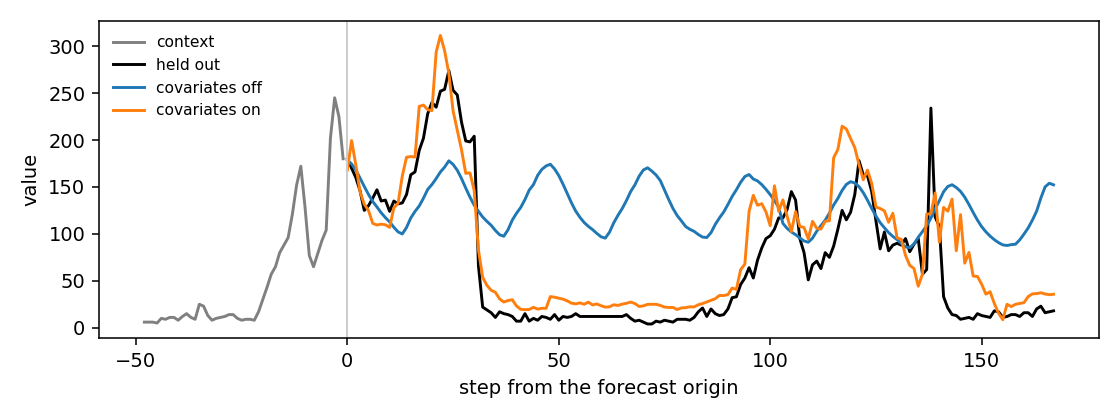
\includegraphics[width=0.92\textwidth]{Task2/outputs/val_last_block.png}
\caption{Last validation block. Grey is context, black is held out, blue is covariates off, orange is covariates on.}
\label{fig:t2val}
\end{figure}

\subsection*{How the forecast improved}

I trained three models and submitted each one. Every comparison was on the same 12 blocks, before anything was pasted to the leaderboard.

\begin{table}[H]
\centering
\small
\begin{tabular}{lrrrrrr}
\toprule
Submission & $P$ & $E$ & Val RMSE & RMSE & MAE & sMAPE (\%) \\
\midrule
Autoformer only & 117,506 & 1 & 85.45 & 82.23 & 66.93 & 74.28 \\
Hourly head added & 33,891 & 12 & 58.78 & 77.75 & 57.07 & 56.73 \\
Day-level correction & 36,900 & 12 & 59.44 & 71.10 & 50.72 & 51.55 \\
\bottomrule
\end{tabular}
\caption{The three submitted models. RMSE, MAE, and sMAPE are the leaderboard scores. Val RMSE is the mean over three seeds, covariates on.}
\end{table}

The first model had the decomposition, the auto-correlation, and the covariates, and nothing else. Width was 64, with two encoder layers. Validation RMSE was 85.45 with covariates and 126.4 without. The learning rate was $10^{-3}$. Validation was best at epoch 1 and then got worse while the training loss kept falling, so the submitted run is one epoch and $P$ is 117,506. Leaderboard RMSE was 82.23, close to validation, so the split was not flattering the model. The forecast mean was about 140, and some hours were clipped to zero. The shape was roughly right. The level was not.

The second model keeps a smaller Autoformer for the seasonal residual and lets the hourly head carry the level. Width is 32, with one layer of each kind. The head is trained at $10^{-3}$ and the Autoformer at $10^{-4}$. Validation RMSE fell to 58.78 with covariates and to about 105 without. The median best epoch was 12, so $E=12$ and $P=33{,}891$. Leaderboard RMSE was 77.75. Better, but 59 on validation and 78 on the leaderboard do not match. The average of the 12 blocks was easier than the week being scored.

That week starts after a very low day. The last 24 training values average about 14. Two of the validation blocks also start after a low day, meaning the previous day averages under 40. The second model did well on ordinary weeks and worse on those two. I also tried a smaller Autoformer with a slower learning rate and no hourly head. Validation RMSE went up to about 96, so I did not submit it.

The final model is the second one with two changes, both inside training. Windows that start after a low day get more weight in the loss, and the loss also matches the seven daily means. The day-level head learns a correction for each of those days. I keep the checkpoint with the better mix of overall RMSE and that clean-start RMSE. Across the three seeds the overall RMSE stays near 59.44, and the clean-start RMSE comes down to 59.07. Leaderboard RMSE is 71.10, MAE is 50.72, and sMAPE is 51.55\%. That is the file in \texttt{Task2/outputs/submission\_168.txt}. It has 36,900 parameters. The run that wrote the file was trained on the full observed history for 12 epochs, the median best epoch of the covariate setting, so $E=12$. The seed search chose that number. It did not produce the submitted weights.

Validation on the clean-start blocks is 59 and the leaderboard score is 71. The test week is still harder than those two blocks. The file is the model's own forecast.

\section*{AI use disclosure}
I used Cursor (Composer) while coding and while drafting this report.

\noindent\textbf{Coding prompts (summary):} implement the three TODO cells; fix local Jupyter/\texttt{ipykernel}; run the notebook on Colab with \texttt{PA1\_PRESET=full}; set up the GitHub repo.

\noindent\textbf{Model help on code:} filled \texttt{forward}, decomposition, and \texttt{aggregate\_delays}; helped with Colab execution and packaging.

\noindent\textbf{My edits on code:} checked shapes against the notebook contracts, kept the worked examples, chose width 41 and the period-routed deployment models from the validation tables myself.

\noindent\textbf{Report prompts (summary):} write Task 1 responses from the full-run CSVs/figures in simple English I can defend in a viva; avoid AI-sounding style. Later, add the Task 2 section from the notebook's validation table and the three leaderboard scores.

\noindent\textbf{Task 2 coding:} Cursor implemented \texttt{Task2/Task2.ipynb} and I ran it on Colab (Tesla T4). I chose the 12-block split, the hourly features, and the day-level loss, and I checked that \texttt{submission\_168.txt} is the model's own forecast.

\noindent\textbf{My edits on the report:} rewrote wording, cut fluff, kept only numbers from my \texttt{full} run and from the Task 2 outputs, and matched Task 1 to the PDF response checklist.

\end{document}
